\documentclass[twoside]{book}

% Packages required by doxygen
\usepackage{fixltx2e}
\usepackage{calc}
\usepackage{doxygen}
\usepackage[export]{adjustbox} % also loads graphicx
\usepackage{graphicx}
\usepackage[utf8]{inputenc}
\usepackage{makeidx}
\usepackage{multicol}
\usepackage{multirow}
\PassOptionsToPackage{warn}{textcomp}
\usepackage{textcomp}
\usepackage[nointegrals]{wasysym}
\usepackage[table]{xcolor}

% Font selection
\usepackage[T1]{fontenc}
\usepackage[scaled=.90]{helvet}
\usepackage{courier}
\usepackage{amssymb}
\usepackage{sectsty}
\renewcommand{\familydefault}{\sfdefault}
\allsectionsfont{%
  \fontseries{bc}\selectfont%
  \color{darkgray}%
}
\renewcommand{\DoxyLabelFont}{%
  \fontseries{bc}\selectfont%
  \color{darkgray}%
}
\newcommand{\+}{\discretionary{\mbox{\scriptsize$\hookleftarrow$}}{}{}}

% Page & text layout
\usepackage{geometry}
\geometry{%
  a4paper,%
  top=2.5cm,%
  bottom=2.5cm,%
  left=2.5cm,%
  right=2.5cm%
}
\tolerance=750
\hfuzz=15pt
\hbadness=750
\setlength{\emergencystretch}{15pt}
\setlength{\parindent}{0cm}
\setlength{\parskip}{3ex plus 2ex minus 2ex}
\makeatletter
\renewcommand{\paragraph}{%
  \@startsection{paragraph}{4}{0ex}{-1.0ex}{1.0ex}{%
    \normalfont\normalsize\bfseries\SS@parafont%
  }%
}
\renewcommand{\subparagraph}{%
  \@startsection{subparagraph}{5}{0ex}{-1.0ex}{1.0ex}{%
    \normalfont\normalsize\bfseries\SS@subparafont%
  }%
}
\makeatother

% Headers & footers
\usepackage{fancyhdr}
\pagestyle{fancyplain}
\fancyhead[LE]{\fancyplain{}{\bfseries\thepage}}
\fancyhead[CE]{\fancyplain{}{}}
\fancyhead[RE]{\fancyplain{}{\bfseries\leftmark}}
\fancyhead[LO]{\fancyplain{}{\bfseries\rightmark}}
\fancyhead[CO]{\fancyplain{}{}}
\fancyhead[RO]{\fancyplain{}{\bfseries\thepage}}
\fancyfoot[LE]{\fancyplain{}{}}
\fancyfoot[CE]{\fancyplain{}{}}
\fancyfoot[RE]{\fancyplain{}{\bfseries\scriptsize Generated by Doxygen }}
\fancyfoot[LO]{\fancyplain{}{\bfseries\scriptsize Generated by Doxygen }}
\fancyfoot[CO]{\fancyplain{}{}}
\fancyfoot[RO]{\fancyplain{}{}}
\renewcommand{\footrulewidth}{0.4pt}
\renewcommand{\chaptermark}[1]{%
  \markboth{#1}{}%
}
\renewcommand{\sectionmark}[1]{%
  \markright{\thesection\ #1}%
}

% Indices & bibliography
\usepackage{natbib}
\usepackage[titles]{tocloft}
\setcounter{tocdepth}{3}
\setcounter{secnumdepth}{5}
\makeindex

% Hyperlinks (required, but should be loaded last)
\usepackage{ifpdf}
\ifpdf
  \usepackage[pdftex,pagebackref=true]{hyperref}
\else
  \usepackage[ps2pdf,pagebackref=true]{hyperref}
\fi
\hypersetup{%
  colorlinks=true,%
  linkcolor=blue,%
  citecolor=blue,%
  unicode%
}

% Custom commands
\newcommand{\clearemptydoublepage}{%
  \newpage{\pagestyle{empty}\cleardoublepage}%
}

\usepackage{caption}
\captionsetup{labelsep=space,justification=centering,font={bf},singlelinecheck=off,skip=4pt,position=top}

%===== C O N T E N T S =====

\begin{document}

% Titlepage & ToC
\hypersetup{pageanchor=false,
             bookmarksnumbered=true,
             pdfencoding=unicode
            }
\pagenumbering{alph}
\begin{titlepage}
\vspace*{7cm}
\begin{center}%
{\Large My Project }\\
\vspace*{1cm}
{\large Generated by Doxygen 1.8.14}\\
\end{center}
\end{titlepage}
\clearemptydoublepage
\pagenumbering{roman}
\tableofcontents
\clearemptydoublepage
\pagenumbering{arabic}
\hypersetup{pageanchor=true}

%--- Begin generated contents ---
\chapter{Hierarchical Index}
\section{Class Hierarchy}
This inheritance list is sorted roughly, but not completely, alphabetically\+:\begin{DoxyCompactList}
\item \contentsline{section}{Button\+Listener}{\pageref{class_button_listener}}{}
\begin{DoxyCompactList}
\item \contentsline{section}{Shoot\+Control}{\pageref{class_shoot_control}}{}
\end{DoxyCompactList}
\item \contentsline{section}{ir\+\_\+msg}{\pageref{structir__msg}}{}
\item \contentsline{section}{I\+R\+Control}{\pageref{class_i_r_control}}{}
\begin{DoxyCompactList}
\item \contentsline{section}{Shoot\+Control}{\pageref{class_shoot_control}}{}
\end{DoxyCompactList}
\item \contentsline{section}{msg\+\_\+listener}{\pageref{classmsg__listener}}{}
\begin{DoxyCompactList}
\item \contentsline{section}{msg\+\_\+logger}{\pageref{classmsg__logger}}{}
\end{DoxyCompactList}
\item \contentsline{section}{pause\+\_\+listener}{\pageref{classpause__listener}}{}
\begin{DoxyCompactList}
\item \contentsline{section}{msg\+\_\+decoder}{\pageref{classmsg__decoder}}{}
\end{DoxyCompactList}
\item task\begin{DoxyCompactList}
\item \contentsline{section}{Button}{\pageref{class_button}}{}
\item \contentsline{section}{msg\+\_\+decoder}{\pageref{classmsg__decoder}}{}
\item \contentsline{section}{msg\+\_\+logger}{\pageref{classmsg__logger}}{}
\item \contentsline{section}{pause\+\_\+detector}{\pageref{classpause__detector}}{}
\item \contentsline{section}{Shoot\+Control}{\pageref{class_shoot_control}}{}
\end{DoxyCompactList}
\end{DoxyCompactList}

\chapter{Class Index}
\section{Class List}
Here are the classes, structs, unions and interfaces with brief descriptions\+:\begin{DoxyCompactList}
\item\contentsline{section}{\mbox{\hyperlink{class_button}{Button}} \\*This class is used to make a button object }{\pageref{class_button}}{}
\item\contentsline{section}{\mbox{\hyperlink{class_button_listener}{Button\+Listener}} \\*A class containing the virtual button\+Pressed function }{\pageref{class_button_listener}}{}
\item\contentsline{section}{\mbox{\hyperlink{class_buzzer_control}{Buzzer\+Control}} \\*This class is used to control the buzzer }{\pageref{class_buzzer_control}}{}
\item\contentsline{section}{\mbox{\hyperlink{class_display_control}{Display\+Control}} \\*This class is used to show the command value on the screen }{\pageref{class_display_control}}{}
\item\contentsline{section}{\mbox{\hyperlink{class_game_leader}{Game\+Leader}} \\*This class is used to make the game }{\pageref{class_game_leader}}{}
\item\contentsline{section}{\mbox{\hyperlink{class_game_logs}{Game\+Logs}} \\*This class is used to track all the hits during the game and to print them at the end }{\pageref{class_game_logs}}{}
\item\contentsline{section}{\mbox{\hyperlink{structir__msg}{ir\+\_\+msg}} \\*This struct gets used to split the message in two parts }{\pageref{structir__msg}}{}
\item\contentsline{section}{\mbox{\hyperlink{class_i_r_control}{I\+R\+Control}} \\*This class is used to control the IR signal }{\pageref{class_i_r_control}}{}
\item\contentsline{section}{\mbox{\hyperlink{class_keypad}{Keypad}} \\*In this class you can find the pin setup and initialize the characters }{\pageref{class_keypad}}{}
\item\contentsline{section}{\mbox{\hyperlink{class_keypad_control}{Keypad\+Control}} \\*This class is used to control the keypad }{\pageref{class_keypad_control}}{}
\item\contentsline{section}{\mbox{\hyperlink{classmsg__decoder}{msg\+\_\+decoder}} }{\pageref{classmsg__decoder}}{}
\item\contentsline{section}{\mbox{\hyperlink{classmsg__listener}{msg\+\_\+listener}} }{\pageref{classmsg__listener}}{}
\item\contentsline{section}{\mbox{\hyperlink{classmsg__logger}{msg\+\_\+logger}} }{\pageref{classmsg__logger}}{}
\item\contentsline{section}{\mbox{\hyperlink{class_msg_decoder}{Msg\+Decoder}} \\*This class decodes the incoming message and sends it to another class }{\pageref{class_msg_decoder}}{}
\item\contentsline{section}{\mbox{\hyperlink{class_msg_listener}{Msg\+Listener}} \\*This class constains the virtual msg\+Received function }{\pageref{class_msg_listener}}{}
\item\contentsline{section}{\mbox{\hyperlink{classpause__detector}{pause\+\_\+detector}} }{\pageref{classpause__detector}}{}
\item\contentsline{section}{\mbox{\hyperlink{classpause__listener}{pause\+\_\+listener}} }{\pageref{classpause__listener}}{}
\item\contentsline{section}{\mbox{\hyperlink{class_pause_detector}{Pause\+Detector}} \\*This class detects the pauses in a IR signal and sends them to another class }{\pageref{class_pause_detector}}{}
\item\contentsline{section}{\mbox{\hyperlink{class_pause_listener}{Pause\+Listener}} \\*This class contains the virtual function pause\+Detected }{\pageref{class_pause_listener}}{}
\item\contentsline{section}{\mbox{\hyperlink{class_player_control}{Player\+Control}} \\*This class controls the player tasks }{\pageref{class_player_control}}{}
\item\contentsline{section}{\mbox{\hyperlink{class_player_data}{Player\+Data}} \\*This class contains all the playerdata }{\pageref{class_player_data}}{}
\item\contentsline{section}{\mbox{\hyperlink{class_send_control}{Send\+Control}} \\*This class is used to send the data }{\pageref{class_send_control}}{}
\item\contentsline{section}{\mbox{\hyperlink{class_shoot_control}{Shoot\+Control}} \\*This class encodes and sends the message to be sent to the \mbox{\hyperlink{class_i_r_control}{I\+R\+Control}} class and controls the laser }{\pageref{class_shoot_control}}{}
\item\contentsline{section}{\mbox{\hyperlink{class_weapon}{Weapon}} \\*This class contains the data of the weapon }{\pageref{class_weapon}}{}
\end{DoxyCompactList}

\chapter{File Index}
\section{File List}
Here is a list of all documented files with brief descriptions\+:\begin{DoxyCompactList}
\item\contentsline{section}{C\+:/ti-\/software/thema\+\_\+opdracht\+\_\+lasergame/\+Player/\mbox{\hyperlink{_button_8hpp}{Button.\+hpp}} }{\pageref{_button_8hpp}}{}
\item\contentsline{section}{C\+:/ti-\/software/thema\+\_\+opdracht\+\_\+lasergame/\+Player/\mbox{\hyperlink{_button_listener_8hpp}{Button\+Listener.\+hpp}} }{\pageref{_button_listener_8hpp}}{}
\item\contentsline{section}{C\+:/ti-\/software/thema\+\_\+opdracht\+\_\+lasergame/\+Player/\mbox{\hyperlink{_buzzer_control_8hpp}{Buzzer\+Control.\+hpp}} }{\pageref{_buzzer_control_8hpp}}{}
\item\contentsline{section}{C\+:/ti-\/software/thema\+\_\+opdracht\+\_\+lasergame/\+Player/\mbox{\hyperlink{_display_control_8hpp}{Display\+Control.\+hpp}} }{\pageref{_display_control_8hpp}}{}
\item\contentsline{section}{C\+:/ti-\/software/thema\+\_\+opdracht\+\_\+lasergame/\+Player/\mbox{\hyperlink{_game_logs_8hpp}{Game\+Logs.\+hpp}} }{\pageref{_game_logs_8hpp}}{}
\item\contentsline{section}{C\+:/ti-\/software/thema\+\_\+opdracht\+\_\+lasergame/\+Player/\mbox{\hyperlink{_i_r_control_8hpp}{I\+R\+Control.\+hpp}} }{\pageref{_i_r_control_8hpp}}{}
\item\contentsline{section}{C\+:/ti-\/software/thema\+\_\+opdracht\+\_\+lasergame/\+Player/\mbox{\hyperlink{_keypad_8hpp}{Keypad.\+hpp}} }{\pageref{_keypad_8hpp}}{}
\item\contentsline{section}{C\+:/ti-\/software/thema\+\_\+opdracht\+\_\+lasergame/\+Player/\mbox{\hyperlink{_keypad_control_8hpp}{Keypad\+Control.\+hpp}} }{\pageref{_keypad_control_8hpp}}{}
\item\contentsline{section}{C\+:/ti-\/software/thema\+\_\+opdracht\+\_\+lasergame/\+Player/\mbox{\hyperlink{_msg_decoder_8hpp}{Msg\+Decoder.\+hpp}} }{\pageref{_msg_decoder_8hpp}}{}
\item\contentsline{section}{C\+:/ti-\/software/thema\+\_\+opdracht\+\_\+lasergame/\+Player/\mbox{\hyperlink{_msg_listener_8hpp}{Msg\+Listener.\+hpp}} }{\pageref{_msg_listener_8hpp}}{}
\item\contentsline{section}{C\+:/ti-\/software/thema\+\_\+opdracht\+\_\+lasergame/\+Player/\mbox{\hyperlink{_pause_detector_8hpp}{Pause\+Detector.\+hpp}} }{\pageref{_pause_detector_8hpp}}{}
\item\contentsline{section}{C\+:/ti-\/software/thema\+\_\+opdracht\+\_\+lasergame/\+Player/\mbox{\hyperlink{_pause_listener_8hpp}{Pause\+Listener.\+hpp}} }{\pageref{_pause_listener_8hpp}}{}
\item\contentsline{section}{C\+:/ti-\/software/thema\+\_\+opdracht\+\_\+lasergame/\+Player/\mbox{\hyperlink{_player_control_8hpp}{Player\+Control.\+hpp}} }{\pageref{_player_control_8hpp}}{}
\item\contentsline{section}{C\+:/ti-\/software/thema\+\_\+opdracht\+\_\+lasergame/\+Player/\mbox{\hyperlink{_player_data_8hpp}{Player\+Data.\+hpp}} }{\pageref{_player_data_8hpp}}{}
\item\contentsline{section}{C\+:/ti-\/software/thema\+\_\+opdracht\+\_\+lasergame/\+Player/\mbox{\hyperlink{_shoot_control_8hpp}{Shoot\+Control.\+hpp}} }{\pageref{_shoot_control_8hpp}}{}
\item\contentsline{section}{C\+:/ti-\/software/thema\+\_\+opdracht\+\_\+lasergame/\+Player/\mbox{\hyperlink{_weapon_8hpp}{Weapon.\+hpp}} }{\pageref{_weapon_8hpp}}{}
\end{DoxyCompactList}

\chapter{Class Documentation}
\hypertarget{class_buzzer_control}{}\section{Buzzer\+Control Class Reference}
\label{class_buzzer_control}\index{Buzzer\+Control@{Buzzer\+Control}}


This class is used to control the buzzer.  




{\ttfamily \#include $<$Buzzer\+Control.\+hpp$>$}

Inheritance diagram for Buzzer\+Control\+:\begin{figure}[H]
\begin{center}
\leavevmode
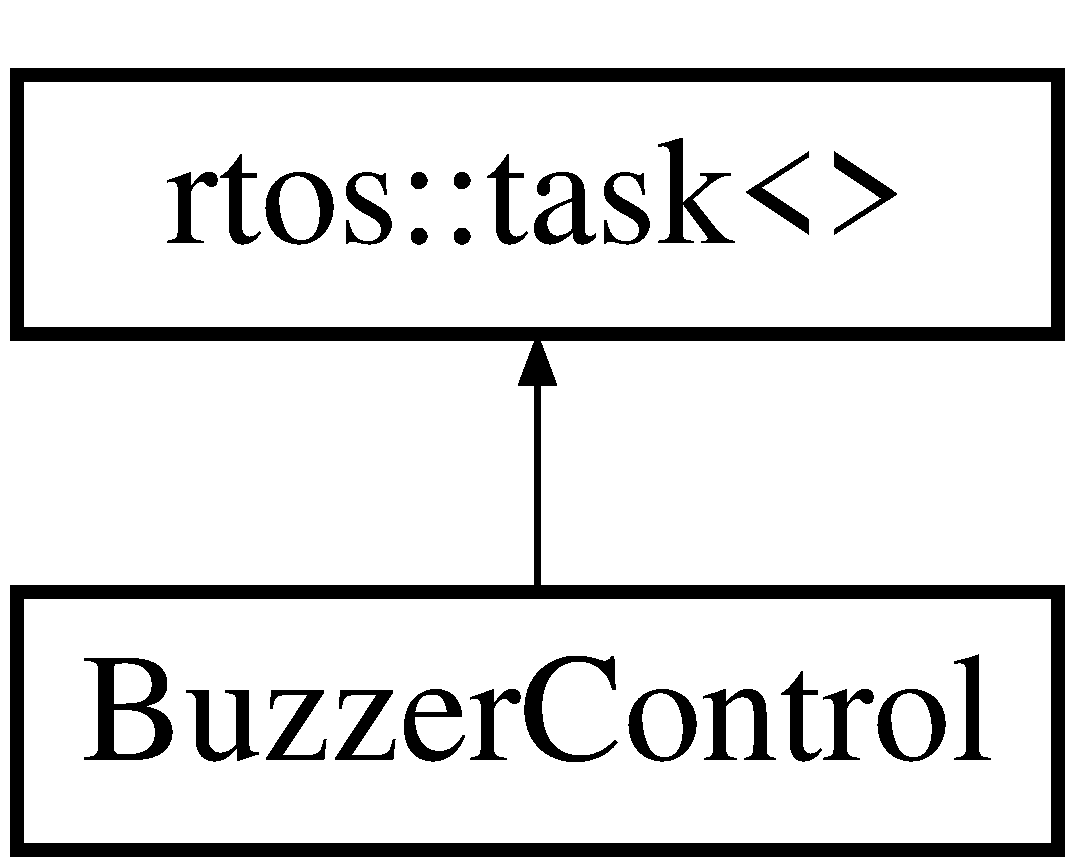
\includegraphics[height=2.000000cm]{class_buzzer_control}
\end{center}
\end{figure}
\subsection*{Public Member Functions}
\begin{DoxyCompactItemize}
\item 
\mbox{\hyperlink{class_buzzer_control_a25b3a51e33513aeeb0beb137463bbe70}{Buzzer\+Control}} (const char $\ast$name, int priority, hwlib\+::pin\+\_\+out \&buzz\+\_\+pin)
\begin{DoxyCompactList}\small\item\em This is the constructer for buzzer control. \end{DoxyCompactList}\item 
\mbox{\Hypertarget{class_buzzer_control_a2c485c8888d861efae8461a87a47685f}\label{class_buzzer_control_a2c485c8888d861efae8461a87a47685f}} 
void \mbox{\hyperlink{class_buzzer_control_a2c485c8888d861efae8461a87a47685f}{make\+Sound}} (int buzz\+\_\+length)
\begin{DoxyCompactList}\small\item\em This function writes the buzz\+\_\+length in the buzz\+\_\+pool and sets the buzz\+\_\+on\+\_\+flag. \end{DoxyCompactList}\item 
void \mbox{\hyperlink{class_buzzer_control_ae249e78ba5c0399e8b14091a0a8254eb}{main}} () override
\begin{DoxyCompactList}\small\item\em This is the state function for the buzzer. \end{DoxyCompactList}\end{DoxyCompactItemize}


\subsection{Detailed Description}
This class is used to control the buzzer. 

\subsection{Constructor \& Destructor Documentation}
\mbox{\Hypertarget{class_buzzer_control_a25b3a51e33513aeeb0beb137463bbe70}\label{class_buzzer_control_a25b3a51e33513aeeb0beb137463bbe70}} 
\index{Buzzer\+Control@{Buzzer\+Control}!Buzzer\+Control@{Buzzer\+Control}}
\index{Buzzer\+Control@{Buzzer\+Control}!Buzzer\+Control@{Buzzer\+Control}}
\subsubsection{\texorpdfstring{Buzzer\+Control()}{BuzzerControl()}}
{\footnotesize\ttfamily Buzzer\+Control\+::\+Buzzer\+Control (\begin{DoxyParamCaption}\item[{const char $\ast$}]{name,  }\item[{int}]{priority,  }\item[{hwlib\+::pin\+\_\+out \&}]{buzz\+\_\+pin }\end{DoxyParamCaption})\hspace{0.3cm}{\ttfamily [inline]}}



This is the constructer for buzzer control. 

The constructer wants a pin\+\_\+out buzz pin. 

\subsection{Member Function Documentation}
\mbox{\Hypertarget{class_buzzer_control_ae249e78ba5c0399e8b14091a0a8254eb}\label{class_buzzer_control_ae249e78ba5c0399e8b14091a0a8254eb}} 
\index{Buzzer\+Control@{Buzzer\+Control}!main@{main}}
\index{main@{main}!Buzzer\+Control@{Buzzer\+Control}}
\subsubsection{\texorpdfstring{main()}{main()}}
{\footnotesize\ttfamily void Buzzer\+Control\+::main (\begin{DoxyParamCaption}{ }\end{DoxyParamCaption})\hspace{0.3cm}{\ttfamily [inline]}, {\ttfamily [override]}}



This is the state function for the buzzer. 

This function has 3 states\+: I\+D\+LE, ON, O\+FF. If the state is I\+D\+LE, the function waits for the buzz\+\_\+on\+\_\+flag, then he reads the buzz\+\_\+pool, set the length timer and switch the state to ON. If the state is ON, buzz\+\_\+pin is set high, interval\+\_\+timer is set, he waits for the buzz\+\_\+interval\+\_\+timer and the state will be O\+FF. If the state is O\+FF, buzz\+\_\+pin is set low, interval\+\_\+timer is set and if event is the same as buzz\+\_\+length\+\_\+timer, the state will be I\+D\+LE. If event is the ame as buzz\+\_\+interval\+\_\+timer, the state will be ON. 

The documentation for this class was generated from the following file\+:\begin{DoxyCompactItemize}
\item 
C\+:/ti-\/software/thema\+\_\+opdracht\+\_\+lasergame/\+Player/\mbox{\hyperlink{_buzzer_control_8hpp}{Buzzer\+Control.\+hpp}}\end{DoxyCompactItemize}

\hypertarget{class_display_control}{}\section{Display\+Control Class Reference}
\label{class_display_control}\index{Display\+Control@{Display\+Control}}


This class is used to show the command value on the screen.  




{\ttfamily \#include $<$Display\+Control.\+hpp$>$}

Inheritance diagram for Display\+Control\+:\begin{figure}[H]
\begin{center}
\leavevmode
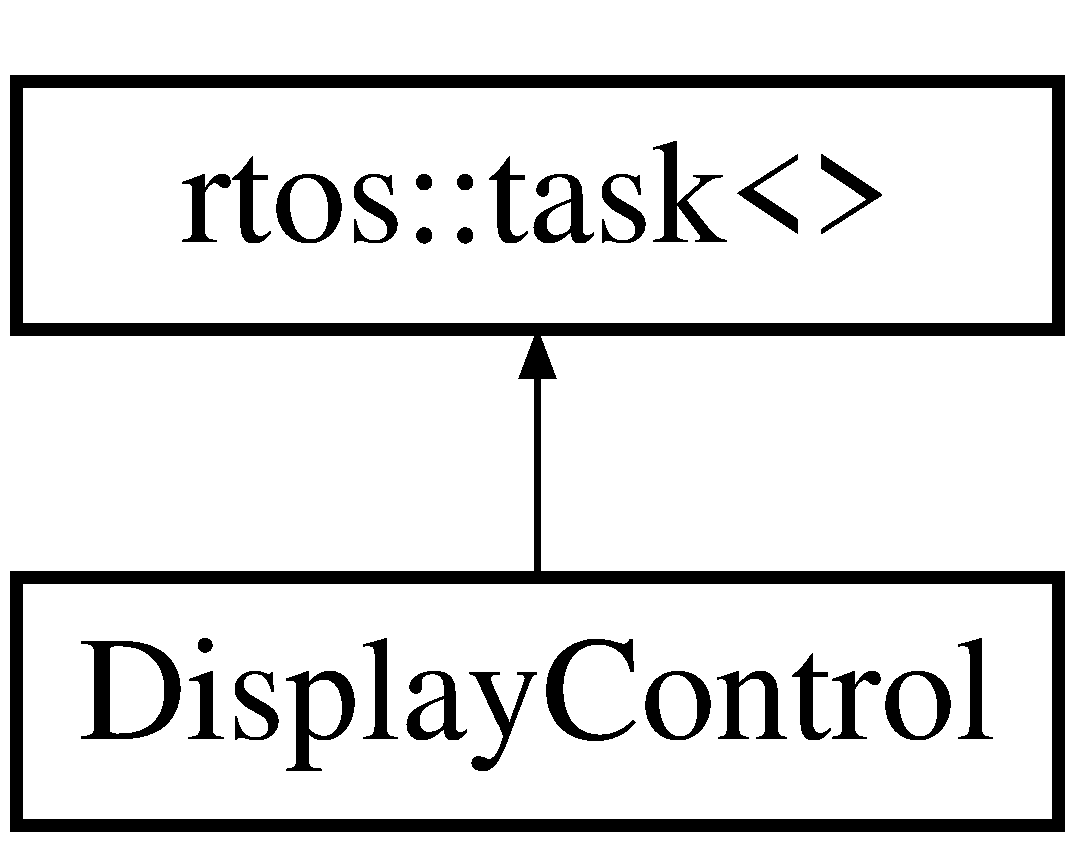
\includegraphics[height=2.000000cm]{class_display_control}
\end{center}
\end{figure}
\subsection*{Public Member Functions}
\begin{DoxyCompactItemize}
\item 
\mbox{\hyperlink{class_display_control_a5a24ccc28d6984bda6871ef6d0e4af3f}{Display\+Control}} (const char $\ast$name, int priority, hwlib\+::glcd\+\_\+oled \&display)
\begin{DoxyCompactList}\small\item\em This is the constructor for a display. \end{DoxyCompactList}\item 
\mbox{\Hypertarget{class_display_control_a78b3ace358fc199a76e00148115f449d}\label{class_display_control_a78b3ace358fc199a76e00148115f449d}} 
void \mbox{\hyperlink{class_display_control_a78b3ace358fc199a76e00148115f449d}{show\+Command}} (uint8\+\_\+t value)
\begin{DoxyCompactList}\small\item\em This function sets a flag en writes the value in the command\+\_\+pool. \end{DoxyCompactList}\item 
\mbox{\Hypertarget{class_display_control_aa231d63d18b09506e0c766999f480579}\label{class_display_control_aa231d63d18b09506e0c766999f480579}} 
void \mbox{\hyperlink{class_display_control_aa231d63d18b09506e0c766999f480579}{clear}} ()
\begin{DoxyCompactList}\small\item\em This function sets a flag to clear the screen. \end{DoxyCompactList}\item 
void \mbox{\hyperlink{class_display_control_ae2d8d0f502941d859639fd46ddd8924b}{update\+Command\+Value}} (uint8\+\_\+t value)
\begin{DoxyCompactList}\small\item\em This function updates the command value on the screen. \end{DoxyCompactList}\item 
\mbox{\Hypertarget{class_display_control_a01207b2034dc3946856496bf2e4d39b6}\label{class_display_control_a01207b2034dc3946856496bf2e4d39b6}} 
void \mbox{\hyperlink{class_display_control_a01207b2034dc3946856496bf2e4d39b6}{clear\+Command\+Value}} ()
\begin{DoxyCompactList}\small\item\em This function clears the command value on the screen. \end{DoxyCompactList}\item 
void \mbox{\hyperlink{class_display_control_a9707c32249e0a648afc2def818900f30}{main}} () override
\begin{DoxyCompactList}\small\item\em This is the state function for the display class. \end{DoxyCompactList}\item 
\mbox{\hyperlink{class_display_control_a5a24ccc28d6984bda6871ef6d0e4af3f}{Display\+Control}} (const char $\ast$name, int priority, hwlib\+::glcd\+\_\+oled \&display)
\begin{DoxyCompactList}\small\item\em This is the constructor for a display. \end{DoxyCompactList}\item 
\mbox{\Hypertarget{class_display_control_a78b3ace358fc199a76e00148115f449d}\label{class_display_control_a78b3ace358fc199a76e00148115f449d}} 
void \mbox{\hyperlink{class_display_control_a78b3ace358fc199a76e00148115f449d}{show\+Command}} (uint8\+\_\+t value)
\begin{DoxyCompactList}\small\item\em This function sets a flag en writes the value in the command\+\_\+pool. \end{DoxyCompactList}\item 
\mbox{\Hypertarget{class_display_control_adcdd7237b9510e9cb9b2aff9d695ad2e}\label{class_display_control_adcdd7237b9510e9cb9b2aff9d695ad2e}} 
void \mbox{\hyperlink{class_display_control_adcdd7237b9510e9cb9b2aff9d695ad2e}{show\+Countdown}} (uint8\+\_\+t value)
\begin{DoxyCompactList}\small\item\em This function sets a flag en writes the value in the countdown\+\_\+pool. \end{DoxyCompactList}\item 
\mbox{\Hypertarget{class_display_control_aee4d1de8dc9b2aab72685cef2ce42d92}\label{class_display_control_aee4d1de8dc9b2aab72685cef2ce42d92}} 
void \mbox{\hyperlink{class_display_control_aee4d1de8dc9b2aab72685cef2ce42d92}{show\+Deaths}} (uint8\+\_\+t value)
\begin{DoxyCompactList}\small\item\em This function sets a flag en writes the value in the deaths\+\_\+pool. \end{DoxyCompactList}\item 
\mbox{\Hypertarget{class_display_control_a6b4ed1ee72406c1ab082b7c6cf900001}\label{class_display_control_a6b4ed1ee72406c1ab082b7c6cf900001}} 
void \mbox{\hyperlink{class_display_control_a6b4ed1ee72406c1ab082b7c6cf900001}{show\+Ammo}} (uint8\+\_\+t value)
\begin{DoxyCompactList}\small\item\em This function sets a flag en writes the value in the ammo\+\_\+pool. \end{DoxyCompactList}\item 
\mbox{\Hypertarget{class_display_control_a4cb0b2e7b72f7267531ffb0470216651}\label{class_display_control_a4cb0b2e7b72f7267531ffb0470216651}} 
void \mbox{\hyperlink{class_display_control_a4cb0b2e7b72f7267531ffb0470216651}{show\+Health}} (uint8\+\_\+t value)
\begin{DoxyCompactList}\small\item\em This function sets a flag en writes the value in the health\+\_\+pool. \end{DoxyCompactList}\item 
\mbox{\Hypertarget{class_display_control_a1f33d5376aee69c307444fef969a1870}\label{class_display_control_a1f33d5376aee69c307444fef969a1870}} 
void \mbox{\hyperlink{class_display_control_a1f33d5376aee69c307444fef969a1870}{show\+Player}} (uint8\+\_\+t value)
\begin{DoxyCompactList}\small\item\em This function sets a flag en writes the value in the player\+\_\+pool. \end{DoxyCompactList}\item 
\mbox{\Hypertarget{class_display_control_a4be28ed55f806917cf4cb7bab68ea6eb}\label{class_display_control_a4be28ed55f806917cf4cb7bab68ea6eb}} 
void \mbox{\hyperlink{class_display_control_a4be28ed55f806917cf4cb7bab68ea6eb}{show\+Weapon}} (const char $\ast$value)
\begin{DoxyCompactList}\small\item\em This function sets a flag en writes the value in the weapon\+\_\+pool. \end{DoxyCompactList}\item 
\mbox{\Hypertarget{class_display_control_ae2d8d0f502941d859639fd46ddd8924b}\label{class_display_control_ae2d8d0f502941d859639fd46ddd8924b}} 
void \mbox{\hyperlink{class_display_control_ae2d8d0f502941d859639fd46ddd8924b}{update\+Command\+Value}} (uint8\+\_\+t value)
\begin{DoxyCompactList}\small\item\em This function updates the command value on the screen. \end{DoxyCompactList}\item 
\mbox{\Hypertarget{class_display_control_a7a566545dbdd6834307d27de99a221d6}\label{class_display_control_a7a566545dbdd6834307d27de99a221d6}} 
void \mbox{\hyperlink{class_display_control_a7a566545dbdd6834307d27de99a221d6}{update\+Countdown\+Value}} (uint8\+\_\+t value)
\begin{DoxyCompactList}\small\item\em This function updates the countdown value on the screen. \end{DoxyCompactList}\item 
\mbox{\Hypertarget{class_display_control_a6bb416767f43144827fa5bf6ecece4a9}\label{class_display_control_a6bb416767f43144827fa5bf6ecece4a9}} 
void \mbox{\hyperlink{class_display_control_a6bb416767f43144827fa5bf6ecece4a9}{update\+Deaths\+Value}} (uint8\+\_\+t value)
\begin{DoxyCompactList}\small\item\em This function updates the deaths value on the screen. \end{DoxyCompactList}\item 
\mbox{\Hypertarget{class_display_control_aa54c7b984287e6a694ea83a3cb3d8ece}\label{class_display_control_aa54c7b984287e6a694ea83a3cb3d8ece}} 
void \mbox{\hyperlink{class_display_control_aa54c7b984287e6a694ea83a3cb3d8ece}{update\+Ammo\+Value}} (uint8\+\_\+t value)
\begin{DoxyCompactList}\small\item\em This function updates the ammo value on the screen. \end{DoxyCompactList}\item 
\mbox{\Hypertarget{class_display_control_a1d61b517063ca3f3dd36d2b7eb3ef909}\label{class_display_control_a1d61b517063ca3f3dd36d2b7eb3ef909}} 
void \mbox{\hyperlink{class_display_control_a1d61b517063ca3f3dd36d2b7eb3ef909}{update\+Healt\+Value}} (uint8\+\_\+t value)
\begin{DoxyCompactList}\small\item\em This function updates the health value on the screen. \end{DoxyCompactList}\item 
\mbox{\Hypertarget{class_display_control_ad6107e04362c907da6a64b73bcc9e795}\label{class_display_control_ad6107e04362c907da6a64b73bcc9e795}} 
void \mbox{\hyperlink{class_display_control_ad6107e04362c907da6a64b73bcc9e795}{update\+Player\+Value}} (uint8\+\_\+t value)
\begin{DoxyCompactList}\small\item\em This function updates the player value on the screen. \end{DoxyCompactList}\item 
\mbox{\Hypertarget{class_display_control_ae343066ad92148ddc6cd9f253993d4b4}\label{class_display_control_ae343066ad92148ddc6cd9f253993d4b4}} 
void \mbox{\hyperlink{class_display_control_ae343066ad92148ddc6cd9f253993d4b4}{update\+Weapon\+Value}} (const char $\ast$value)
\begin{DoxyCompactList}\small\item\em This function updates the weapon value on the screen. \end{DoxyCompactList}\item 
void \mbox{\hyperlink{class_display_control_a9707c32249e0a648afc2def818900f30}{main}} () override
\begin{DoxyCompactList}\small\item\em This is the state function for the display class. \end{DoxyCompactList}\end{DoxyCompactItemize}


\subsection{Detailed Description}
This class is used to show the command value on the screen. 

\subsection{Constructor \& Destructor Documentation}
\mbox{\Hypertarget{class_display_control_a5a24ccc28d6984bda6871ef6d0e4af3f}\label{class_display_control_a5a24ccc28d6984bda6871ef6d0e4af3f}} 
\index{Display\+Control@{Display\+Control}!Display\+Control@{Display\+Control}}
\index{Display\+Control@{Display\+Control}!Display\+Control@{Display\+Control}}
\subsubsection{\texorpdfstring{Display\+Control()}{DisplayControl()}\hspace{0.1cm}{\footnotesize\ttfamily [1/2]}}
{\footnotesize\ttfamily Display\+Control\+::\+Display\+Control (\begin{DoxyParamCaption}\item[{const char $\ast$}]{name,  }\item[{int}]{priority,  }\item[{hwlib\+::glcd\+\_\+oled \&}]{display }\end{DoxyParamCaption})\hspace{0.3cm}{\ttfamily [inline]}}



This is the constructor for a display. 

The constructor expects a display. \mbox{\Hypertarget{class_display_control_a5a24ccc28d6984bda6871ef6d0e4af3f}\label{class_display_control_a5a24ccc28d6984bda6871ef6d0e4af3f}} 
\index{Display\+Control@{Display\+Control}!Display\+Control@{Display\+Control}}
\index{Display\+Control@{Display\+Control}!Display\+Control@{Display\+Control}}
\subsubsection{\texorpdfstring{Display\+Control()}{DisplayControl()}\hspace{0.1cm}{\footnotesize\ttfamily [2/2]}}
{\footnotesize\ttfamily Display\+Control\+::\+Display\+Control (\begin{DoxyParamCaption}\item[{const char $\ast$}]{name,  }\item[{int}]{priority,  }\item[{hwlib\+::glcd\+\_\+oled \&}]{display }\end{DoxyParamCaption})\hspace{0.3cm}{\ttfamily [inline]}}



This is the constructor for a display. 

The constructor expects a display. 

\subsection{Member Function Documentation}
\mbox{\Hypertarget{class_display_control_a9707c32249e0a648afc2def818900f30}\label{class_display_control_a9707c32249e0a648afc2def818900f30}} 
\index{Display\+Control@{Display\+Control}!main@{main}}
\index{main@{main}!Display\+Control@{Display\+Control}}
\subsubsection{\texorpdfstring{main()}{main()}\hspace{0.1cm}{\footnotesize\ttfamily [1/2]}}
{\footnotesize\ttfamily void Display\+Control\+::main (\begin{DoxyParamCaption}{ }\end{DoxyParamCaption})\hspace{0.3cm}{\ttfamily [inline]}, {\ttfamily [override]}}



This is the state function for the display class. 

This function has one state\+: W\+A\+I\+T\+\_\+\+F\+O\+R\+\_\+\+M\+E\+S\+S\+A\+GE. The function will wait for the display\+\_\+command\+\_\+flag and will wait and call a function where he will read the pool. Else if he will wait for the clear\+\_\+flag and will call a function. \mbox{\Hypertarget{class_display_control_a9707c32249e0a648afc2def818900f30}\label{class_display_control_a9707c32249e0a648afc2def818900f30}} 
\index{Display\+Control@{Display\+Control}!main@{main}}
\index{main@{main}!Display\+Control@{Display\+Control}}
\subsubsection{\texorpdfstring{main()}{main()}\hspace{0.1cm}{\footnotesize\ttfamily [2/2]}}
{\footnotesize\ttfamily void Display\+Control\+::main (\begin{DoxyParamCaption}{ }\end{DoxyParamCaption})\hspace{0.3cm}{\ttfamily [inline]}, {\ttfamily [override]}}



This is the state function for the display class. 

This function has one state\+: W\+A\+I\+T\+\_\+\+F\+O\+R\+\_\+\+M\+E\+S\+S\+A\+GE. If event is the same as display\+\_\+command\+\_\+flag, the function update\+Command\+Value with as parameter the readen comman\+\_\+pool value. If event is the same as display\+\_\+countdown\+\_\+flag, the function update\+Countdown\+Value with as parameter the readen countdown\+\_\+pool value. If event is the same as display\+\_\+deaths\+\_\+flag, the function update\+Deaths\+Value with as parameter the readen deaths\+\_\+pool value. If event is the same as display\+\_\+ammo\+\_\+flag, the function update\+Ammo\+Value with as parameter the readen ammo\+\_\+pool value. If event is the same as display\+\_\+health\+\_\+flag, the function update\+Health\+Value with as parameter the readen health\+\_\+pool value. If event is the same as display\+\_\+player\+\_\+flag, the function update\+Player\+Value with as parameter the readen player\+\_\+pool value. If event is the same as display\+\_\+weapon\+\_\+flag, the function update\+Weapon\+Value with as parameter the readen Weapon\+\_\+pool value. \mbox{\Hypertarget{class_display_control_ae2d8d0f502941d859639fd46ddd8924b}\label{class_display_control_ae2d8d0f502941d859639fd46ddd8924b}} 
\index{Display\+Control@{Display\+Control}!update\+Command\+Value@{update\+Command\+Value}}
\index{update\+Command\+Value@{update\+Command\+Value}!Display\+Control@{Display\+Control}}
\subsubsection{\texorpdfstring{update\+Command\+Value()}{updateCommandValue()}}
{\footnotesize\ttfamily void Display\+Control\+::update\+Command\+Value (\begin{DoxyParamCaption}\item[{uint8\+\_\+t}]{value }\end{DoxyParamCaption})\hspace{0.3cm}{\ttfamily [inline]}}



This function updates the command value on the screen. 

If the value is 42, the function makes a star of it. This is special for the star on the gamepad. Else the function will print the int value on the screen. 

The documentation for this class was generated from the following file\+:\begin{DoxyCompactItemize}
\item 
C\+:/ti-\/software/thema\+\_\+opdracht\+\_\+lasergame/\+Gameleader/\mbox{\hyperlink{_gameleader_2_display_control_8hpp}{Display\+Control.\+hpp}}\end{DoxyCompactItemize}

\hypertarget{class_game_leader}{}\section{Game\+Leader Class Reference}
\label{class_game_leader}\index{Game\+Leader@{Game\+Leader}}


This class is used to make the game.  




{\ttfamily \#include $<$Game\+Leader.\+hpp$>$}

Inheritance diagram for Game\+Leader\+:\begin{figure}[H]
\begin{center}
\leavevmode
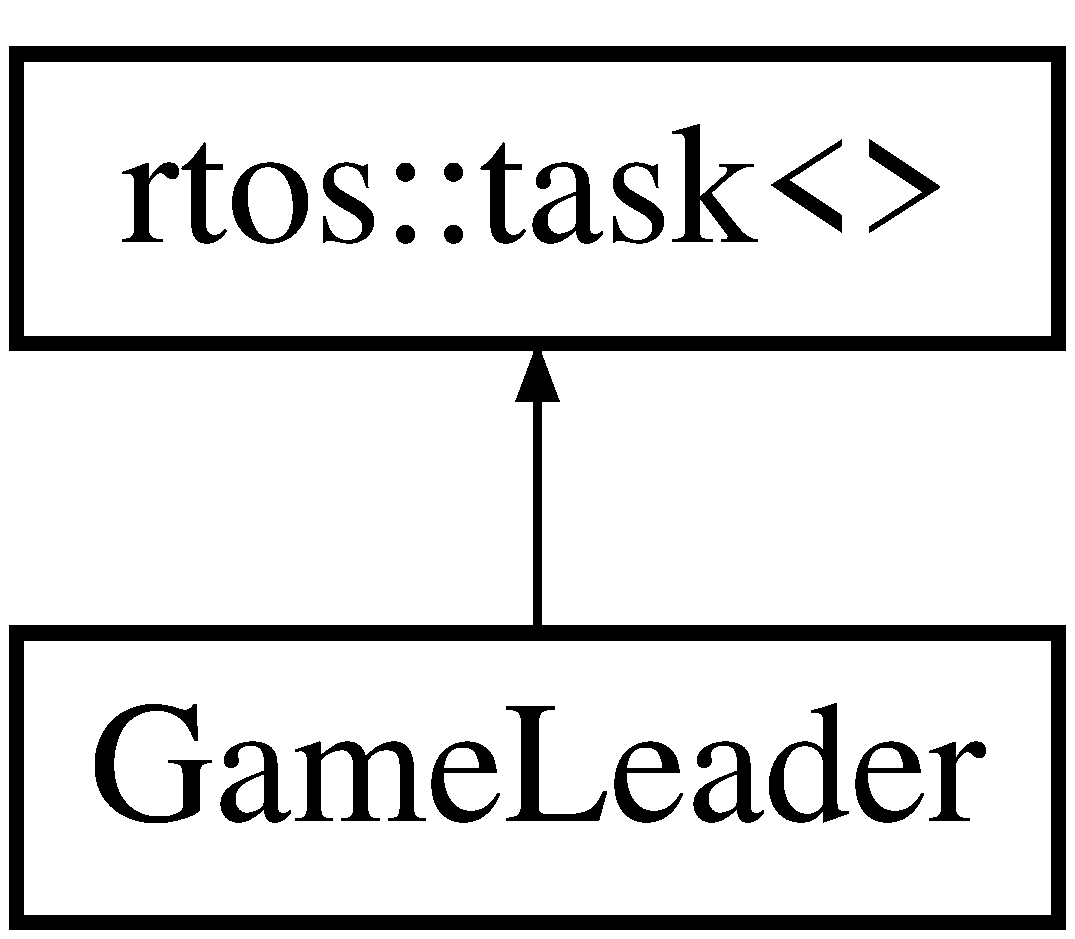
\includegraphics[height=2.000000cm]{class_game_leader}
\end{center}
\end{figure}
\subsection*{Public Member Functions}
\begin{DoxyCompactItemize}
\item 
\mbox{\hyperlink{class_game_leader_a37f89b9731c43cb875207ebbbcdcc96f}{Game\+Leader}} (const char $\ast$name, int priority, \mbox{\hyperlink{class_send_control}{Send\+Control}} \&send\+\_\+control)
\begin{DoxyCompactList}\small\item\em This is the constructor for the \mbox{\hyperlink{class_game_leader}{Game\+Leader}}. \end{DoxyCompactList}\item 
\mbox{\Hypertarget{class_game_leader_a704a13665a65f4528ed3022111c468e2}\label{class_game_leader_a704a13665a65f4528ed3022111c468e2}} 
void \mbox{\hyperlink{class_game_leader_a704a13665a65f4528ed3022111c468e2}{set\+Game\+Length}} (uint8\+\_\+t length)
\begin{DoxyCompactList}\small\item\em This function writes the given length in the game\+\_\+length\+\_\+pool and sets the game\+\_\+length\+\_\+flag. \end{DoxyCompactList}\item 
\mbox{\Hypertarget{class_game_leader_a42849b606a56928126bc915b56695b38}\label{class_game_leader_a42849b606a56928126bc915b56695b38}} 
void \mbox{\hyperlink{class_game_leader_a42849b606a56928126bc915b56695b38}{start\+Game}} ()
\begin{DoxyCompactList}\small\item\em This function sets the start\+\_\+game\+\_\+flag. \end{DoxyCompactList}\item 
void \mbox{\hyperlink{class_game_leader_a83c1a53edf86e4a740c6e4a08f022f36}{main}} () override
\begin{DoxyCompactList}\small\item\em This is the state function for the \mbox{\hyperlink{class_game_leader}{Game\+Leader}} class. \end{DoxyCompactList}\end{DoxyCompactItemize}


\subsection{Detailed Description}
This class is used to make the game. 

\subsection{Constructor \& Destructor Documentation}
\mbox{\Hypertarget{class_game_leader_a37f89b9731c43cb875207ebbbcdcc96f}\label{class_game_leader_a37f89b9731c43cb875207ebbbcdcc96f}} 
\index{Game\+Leader@{Game\+Leader}!Game\+Leader@{Game\+Leader}}
\index{Game\+Leader@{Game\+Leader}!Game\+Leader@{Game\+Leader}}
\subsubsection{\texorpdfstring{Game\+Leader()}{GameLeader()}}
{\footnotesize\ttfamily Game\+Leader\+::\+Game\+Leader (\begin{DoxyParamCaption}\item[{const char $\ast$}]{name,  }\item[{int}]{priority,  }\item[{\mbox{\hyperlink{class_send_control}{Send\+Control}} \&}]{send\+\_\+control }\end{DoxyParamCaption})\hspace{0.3cm}{\ttfamily [inline]}}



This is the constructor for the \mbox{\hyperlink{class_game_leader}{Game\+Leader}}. 

The constructor expects a \mbox{\hyperlink{class_send_control}{Send\+Control}} as parameter. 

\subsection{Member Function Documentation}
\mbox{\Hypertarget{class_game_leader_a83c1a53edf86e4a740c6e4a08f022f36}\label{class_game_leader_a83c1a53edf86e4a740c6e4a08f022f36}} 
\index{Game\+Leader@{Game\+Leader}!main@{main}}
\index{main@{main}!Game\+Leader@{Game\+Leader}}
\subsubsection{\texorpdfstring{main()}{main()}}
{\footnotesize\ttfamily void Game\+Leader\+::main (\begin{DoxyParamCaption}{ }\end{DoxyParamCaption})\hspace{0.3cm}{\ttfamily [inline]}, {\ttfamily [override]}}



This is the state function for the \mbox{\hyperlink{class_game_leader}{Game\+Leader}} class. 

This function has one state\+: W\+A\+I\+T\+I\+N\+G\+\_\+\+F\+O\+R\+\_\+\+C\+O\+M\+M\+A\+ND. The function waits for game\+\_\+length\+\_\+flag and then he will send the value in the game\+\_\+length\+\_\+pool. Else he will wait for the start\+\_\+game\+\_\+flag en then he will send the start\+\_\+game\+\_\+value. 

The documentation for this class was generated from the following file\+:\begin{DoxyCompactItemize}
\item 
C\+:/ti-\/software/thema\+\_\+opdracht\+\_\+lasergame/\+Gameleader/\mbox{\hyperlink{_game_leader_8hpp}{Game\+Leader.\+hpp}}\end{DoxyCompactItemize}

\hypertarget{class_game_logs}{}\section{Game\+Logs Class Reference}
\label{class_game_logs}\index{Game\+Logs@{Game\+Logs}}
\subsection*{Public Member Functions}
\begin{DoxyCompactItemize}
\item 
\mbox{\Hypertarget{class_game_logs_aff50867c6abefacf3d80180015f94e70}\label{class_game_logs_aff50867c6abefacf3d80180015f94e70}} 
void {\bfseries add\+Log} (uint8\+\_\+t player, const char $\ast$weapon)
\item 
\mbox{\Hypertarget{class_game_logs_a2af40236b4dc804f4dc0fac938d0bfd9}\label{class_game_logs_a2af40236b4dc804f4dc0fac938d0bfd9}} 
void {\bfseries print\+Log} ()
\item 
\mbox{\Hypertarget{class_game_logs_ab645b6718f2d5ee716c8b4df4dddf561}\label{class_game_logs_ab645b6718f2d5ee716c8b4df4dddf561}} 
void {\bfseries clear\+Logs} ()
\end{DoxyCompactItemize}


The documentation for this class was generated from the following file\+:\begin{DoxyCompactItemize}
\item 
C\+:/ti-\/software/thema\+\_\+opdracht\+\_\+lasergame/\+Gameleader/Game\+Logs.\+hpp\end{DoxyCompactItemize}

\hypertarget{class_i_r_control}{}\section{I\+R\+Control Class Reference}
\label{class_i_r_control}\index{I\+R\+Control@{I\+R\+Control}}
Inheritance diagram for I\+R\+Control\+:\begin{figure}[H]
\begin{center}
\leavevmode
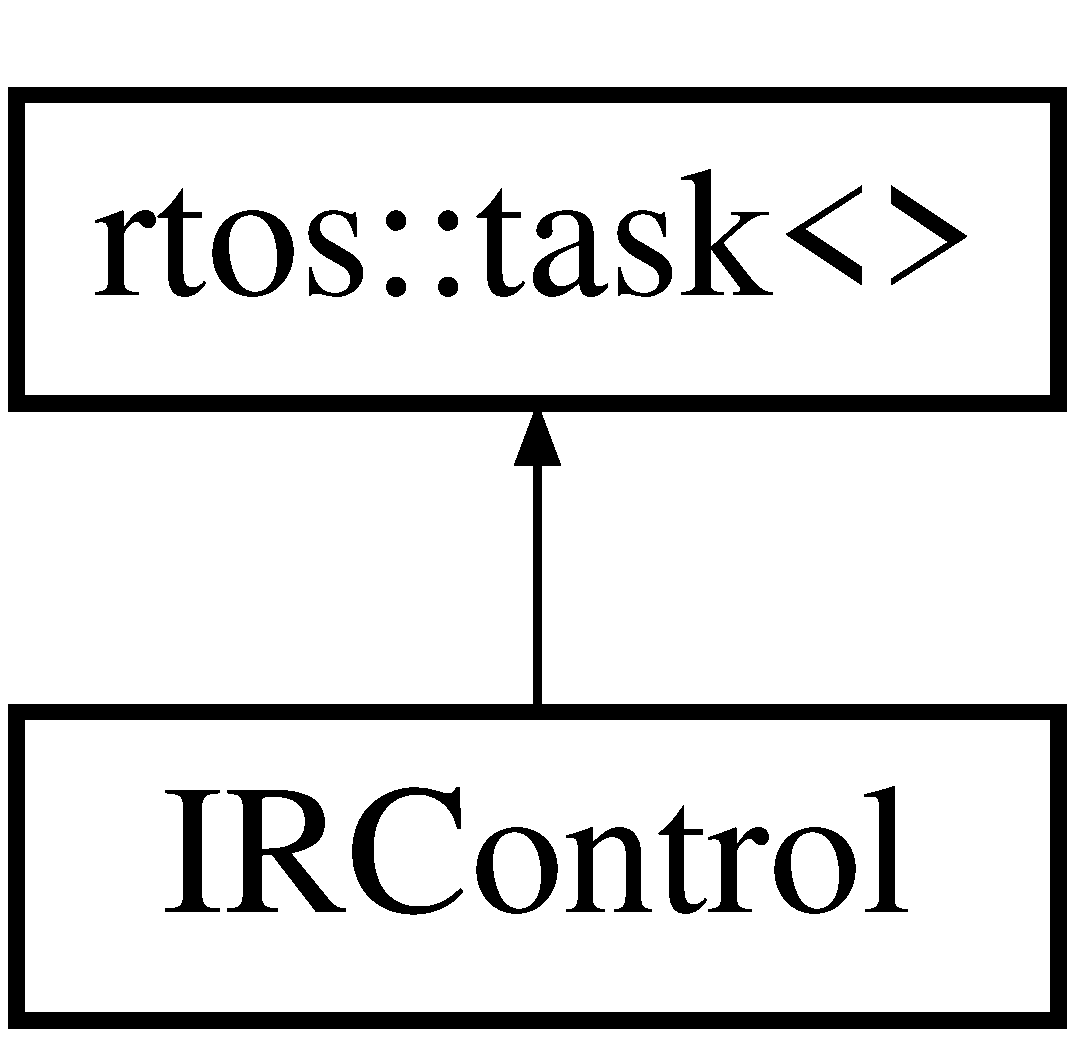
\includegraphics[height=2.000000cm]{class_i_r_control}
\end{center}
\end{figure}
\subsection*{Public Member Functions}
\begin{DoxyCompactItemize}
\item 
\mbox{\Hypertarget{class_i_r_control_ac16a197b453b4bd18874dbc1ef2d3cf4}\label{class_i_r_control_ac16a197b453b4bd18874dbc1ef2d3cf4}} 
void {\bfseries send} (const uint16\+\_\+t \&data)
\item 
\mbox{\Hypertarget{class_i_r_control_a12e0082a899fc811fa70c5cbe59e18d0}\label{class_i_r_control_a12e0082a899fc811fa70c5cbe59e18d0}} 
void {\bfseries pulse} (bool data)
\end{DoxyCompactItemize}


The documentation for this class was generated from the following file\+:\begin{DoxyCompactItemize}
\item 
C\+:/ti-\/software/thema\+\_\+opdracht\+\_\+lasergame/\+I\+R\+\_\+send/I\+R\+Control.\+hpp\end{DoxyCompactItemize}

\hypertarget{class_keypad}{}\section{Keypad Class Reference}
\label{class_keypad}\index{Keypad@{Keypad}}


In this class you can find the pin setup and initialize the characters.  




{\ttfamily \#include $<$Keypad.\+hpp$>$}

Inheritance diagram for Keypad\+:\begin{figure}[H]
\begin{center}
\leavevmode
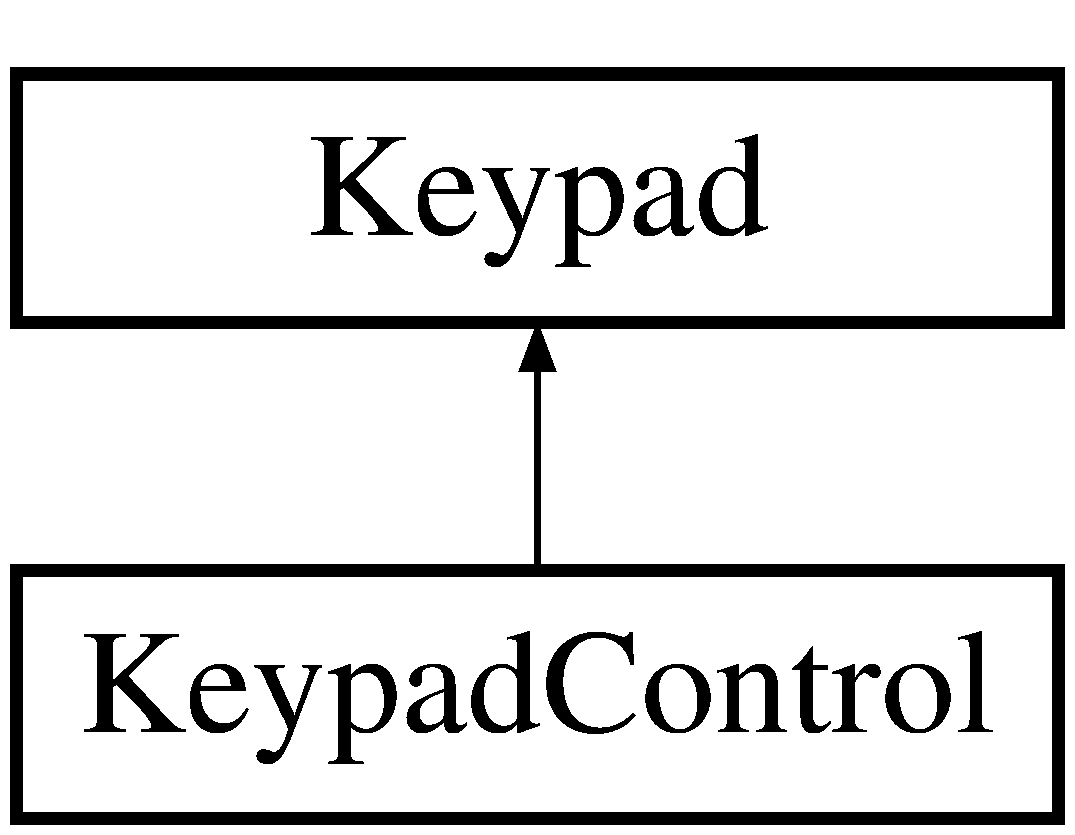
\includegraphics[height=2.000000cm]{class_keypad}
\end{center}
\end{figure}
\subsection*{Public Member Functions}
\begin{DoxyCompactItemize}
\item 
\mbox{\Hypertarget{class_keypad_ade2df731c6751f21bbf745b276cb7208}\label{class_keypad_ade2df731c6751f21bbf745b276cb7208}} 
char \mbox{\hyperlink{class_keypad_ade2df731c6751f21bbf745b276cb7208}{getc}} ()
\begin{DoxyCompactList}\small\item\em This function returns the pressed character. \end{DoxyCompactList}\end{DoxyCompactItemize}


\subsection{Detailed Description}
In this class you can find the pin setup and initialize the characters. 

The documentation for this class was generated from the following file\+:\begin{DoxyCompactItemize}
\item 
C\+:/ti-\/software/thema\+\_\+opdracht\+\_\+lasergame/\+Player/\mbox{\hyperlink{_keypad_8hpp}{Keypad.\+hpp}}\end{DoxyCompactItemize}

\hypertarget{class_keypad_control}{}\section{Keypad\+Control Class Reference}
\label{class_keypad_control}\index{Keypad\+Control@{Keypad\+Control}}


This class is used to control the keypad.  




{\ttfamily \#include $<$Keypad\+Control.\+hpp$>$}

Inheritance diagram for Keypad\+Control\+:\begin{figure}[H]
\begin{center}
\leavevmode
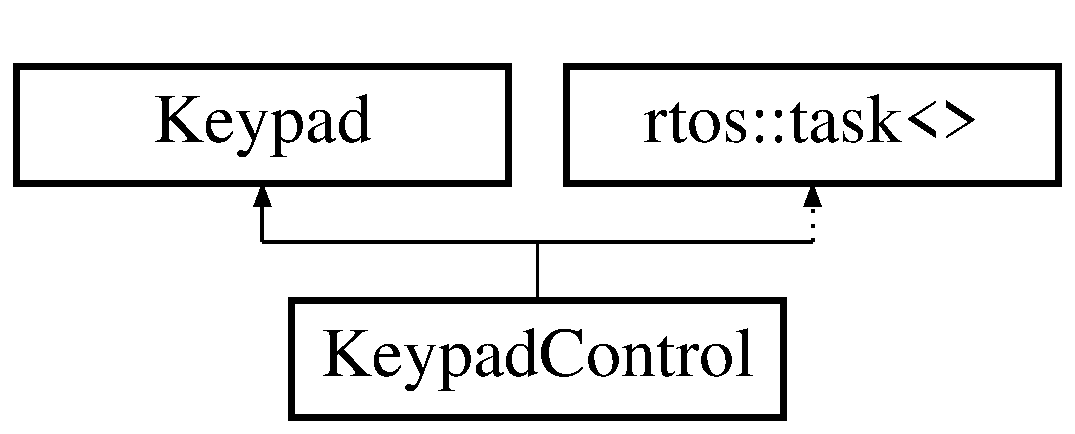
\includegraphics[height=2.000000cm]{class_keypad_control}
\end{center}
\end{figure}
\subsection*{Public Member Functions}
\begin{DoxyCompactItemize}
\item 
\mbox{\hyperlink{class_keypad_control_a4de1bb3018f819011222461d64aa2d67}{Keypad\+Control}} (const char $\ast$name, int priority, \mbox{\hyperlink{class_display_control}{Display\+Control}} \&display\+\_\+control, \mbox{\hyperlink{class_player_control}{Player\+Control}} \&player\+\_\+control, \mbox{\hyperlink{class_weapon}{Weapon}} \&weapon, \mbox{\hyperlink{class_player_data}{Player\+Data}} \&player\+\_\+data)
\begin{DoxyCompactList}\small\item\em This is the constructor for keypad control. \end{DoxyCompactList}\item 
void \mbox{\hyperlink{class_keypad_control_a66ec8a33eceb20d5d1d243c270c3718b}{main}} () override
\begin{DoxyCompactList}\small\item\em This is the state function for the keypad class. \end{DoxyCompactList}\end{DoxyCompactItemize}


\subsection{Detailed Description}
This class is used to control the keypad. 

\subsection{Constructor \& Destructor Documentation}
\mbox{\Hypertarget{class_keypad_control_a4de1bb3018f819011222461d64aa2d67}\label{class_keypad_control_a4de1bb3018f819011222461d64aa2d67}} 
\index{Keypad\+Control@{Keypad\+Control}!Keypad\+Control@{Keypad\+Control}}
\index{Keypad\+Control@{Keypad\+Control}!Keypad\+Control@{Keypad\+Control}}
\subsubsection{\texorpdfstring{Keypad\+Control()}{KeypadControl()}}
{\footnotesize\ttfamily Keypad\+Control\+::\+Keypad\+Control (\begin{DoxyParamCaption}\item[{const char $\ast$}]{name,  }\item[{int}]{priority,  }\item[{\mbox{\hyperlink{class_display_control}{Display\+Control}} \&}]{display\+\_\+control,  }\item[{\mbox{\hyperlink{class_player_control}{Player\+Control}} \&}]{player\+\_\+control,  }\item[{\mbox{\hyperlink{class_weapon}{Weapon}} \&}]{weapon,  }\item[{\mbox{\hyperlink{class_player_data}{Player\+Data}} \&}]{player\+\_\+data }\end{DoxyParamCaption})\hspace{0.3cm}{\ttfamily [inline]}}



This is the constructor for keypad control. 

The constructor needs \mbox{\hyperlink{class_display_control}{Display\+Control}}, \mbox{\hyperlink{class_player_control}{Player\+Control}}, \mbox{\hyperlink{class_weapon}{Weapon}}, \mbox{\hyperlink{class_player_data}{Player\+Data}}. 

\subsection{Member Function Documentation}
\mbox{\Hypertarget{class_keypad_control_a66ec8a33eceb20d5d1d243c270c3718b}\label{class_keypad_control_a66ec8a33eceb20d5d1d243c270c3718b}} 
\index{Keypad\+Control@{Keypad\+Control}!main@{main}}
\index{main@{main}!Keypad\+Control@{Keypad\+Control}}
\subsubsection{\texorpdfstring{main()}{main()}}
{\footnotesize\ttfamily void Keypad\+Control\+::main (\begin{DoxyParamCaption}{ }\end{DoxyParamCaption})\hspace{0.3cm}{\ttfamily [inline]}, {\ttfamily [override]}}



This is the state function for the keypad class. 

This function has 3 states\+: I\+D\+LE, P\+L\+A\+Y\+ER and W\+E\+A\+P\+ON. If the state is I\+D\+LE, the function waits for the receive\+\_\+clock and will look for the pressed key.\+If the pressed key is A then the state will be P\+L\+A\+Y\+ER. Else if the pressed key is B, the state will be W\+E\+A\+P\+ON. If the state is P\+L\+A\+Y\+ER, the function waits for the receive\+\_\+clock and will look for the pressed key. If keyvalue is a number but not 0, the set\+Player\+Number and Show\+Command functions will be called and the state will be I\+D\+LE. If state is W\+E\+A\+P\+ON, the function will wait for the receive\+\_\+clock and will look for the pressed key. If keyvalue is a number but not 0, the set\+Weapon and show\+Command functions will be called and the state will be I\+D\+LE. 

The documentation for this class was generated from the following file\+:\begin{DoxyCompactItemize}
\item 
C\+:/ti-\/software/thema\+\_\+opdracht\+\_\+lasergame/\+Player/\mbox{\hyperlink{_keypad_control_8hpp}{Keypad\+Control.\+hpp}}\end{DoxyCompactItemize}

\hypertarget{class_send_control}{}\section{Send\+Control Class Reference}
\label{class_send_control}\index{Send\+Control@{Send\+Control}}


This class is used to send the data.  




{\ttfamily \#include $<$Send\+Control.\+hpp$>$}

Inheritance diagram for Send\+Control\+:\begin{figure}[H]
\begin{center}
\leavevmode
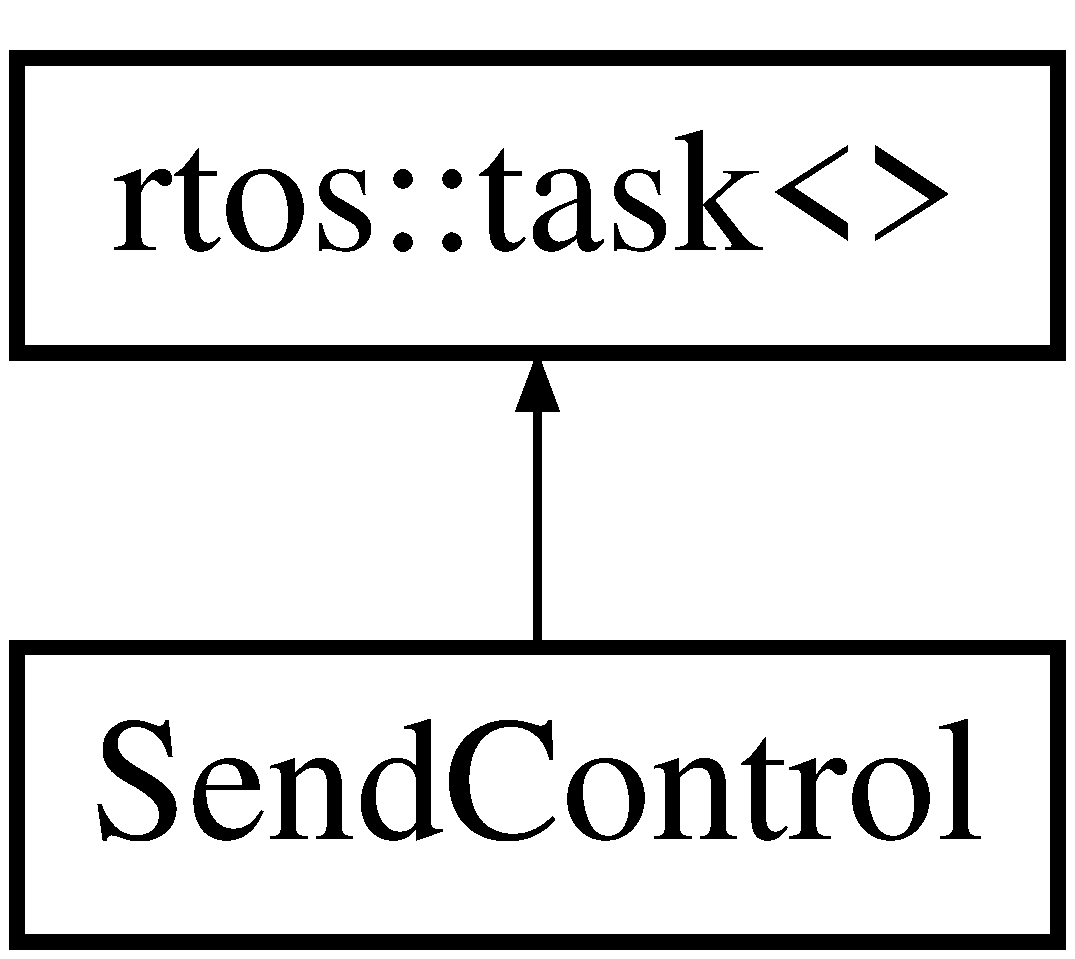
\includegraphics[height=2.000000cm]{class_send_control}
\end{center}
\end{figure}
\subsection*{Public Member Functions}
\begin{DoxyCompactItemize}
\item 
\mbox{\hyperlink{class_send_control_af666c41a0c262bf86bbb3009003b2c81}{Send\+Control}} (const char $\ast$name, int priority, \mbox{\hyperlink{class_i_r_control}{I\+R\+Control}} \&I\+R\+\_\+control)
\begin{DoxyCompactList}\small\item\em This is the constructer of send control. \end{DoxyCompactList}\item 
\mbox{\Hypertarget{class_send_control_a631b78165c258e5ee4bde7d0790385a0}\label{class_send_control_a631b78165c258e5ee4bde7d0790385a0}} 
void \mbox{\hyperlink{class_send_control_a631b78165c258e5ee4bde7d0790385a0}{send}} (uint8\+\_\+t data)
\begin{DoxyCompactList}\small\item\em This function writes the data in the send\+\_\+pool and sets the send\+\_\+flag. \end{DoxyCompactList}\item 
void \mbox{\hyperlink{class_send_control_aedec285713d090002e2848228cef2617}{main}} () override
\begin{DoxyCompactList}\small\item\em This is the state function for send control. \end{DoxyCompactList}\end{DoxyCompactItemize}


\subsection{Detailed Description}
This class is used to send the data. 

\subsection{Constructor \& Destructor Documentation}
\mbox{\Hypertarget{class_send_control_af666c41a0c262bf86bbb3009003b2c81}\label{class_send_control_af666c41a0c262bf86bbb3009003b2c81}} 
\index{Send\+Control@{Send\+Control}!Send\+Control@{Send\+Control}}
\index{Send\+Control@{Send\+Control}!Send\+Control@{Send\+Control}}
\subsubsection{\texorpdfstring{Send\+Control()}{SendControl()}}
{\footnotesize\ttfamily Send\+Control\+::\+Send\+Control (\begin{DoxyParamCaption}\item[{const char $\ast$}]{name,  }\item[{int}]{priority,  }\item[{\mbox{\hyperlink{class_i_r_control}{I\+R\+Control}} \&}]{I\+R\+\_\+control }\end{DoxyParamCaption})\hspace{0.3cm}{\ttfamily [inline]}}



This is the constructer of send control. 

The constructer wants IR control. 

\subsection{Member Function Documentation}
\mbox{\Hypertarget{class_send_control_aedec285713d090002e2848228cef2617}\label{class_send_control_aedec285713d090002e2848228cef2617}} 
\index{Send\+Control@{Send\+Control}!main@{main}}
\index{main@{main}!Send\+Control@{Send\+Control}}
\subsubsection{\texorpdfstring{main()}{main()}}
{\footnotesize\ttfamily void Send\+Control\+::main (\begin{DoxyParamCaption}{ }\end{DoxyParamCaption})\hspace{0.3cm}{\ttfamily [inline]}, {\ttfamily [override]}}



This is the state function for send control. 

This function has 1 state\+: I\+D\+LE. The function waits for the send\+\_\+flag and the call the set\+Send\+Data with as parameter an encoded game\+\_\+leader with send\+\_\+pool readed data. 

The documentation for this class was generated from the following file\+:\begin{DoxyCompactItemize}
\item 
C\+:/ti-\/software/thema\+\_\+opdracht\+\_\+lasergame/\+Gameleader/\mbox{\hyperlink{_send_control_8hpp}{Send\+Control.\+hpp}}\end{DoxyCompactItemize}

\chapter{File Documentation}
\hypertarget{_buzzer_control_8hpp}{}\section{C\+:/ti-\/software/thema\+\_\+opdracht\+\_\+lasergame/\+Gameleader/\+Buzzer\+Control.hpp File Reference}
\label{_buzzer_control_8hpp}\index{C\+:/ti-\/software/thema\+\_\+opdracht\+\_\+lasergame/\+Gameleader/\+Buzzer\+Control.\+hpp@{C\+:/ti-\/software/thema\+\_\+opdracht\+\_\+lasergame/\+Gameleader/\+Buzzer\+Control.\+hpp}}
{\ttfamily \#include \char`\"{}hwlib.\+hpp\char`\"{}}\newline
{\ttfamily \#include \char`\"{}rtos.\+hpp\char`\"{}}\newline
\subsection*{Classes}
\begin{DoxyCompactItemize}
\item 
class \mbox{\hyperlink{class_buzzer_control}{Buzzer\+Control}}
\begin{DoxyCompactList}\small\item\em This class is used to control the buzzer. \end{DoxyCompactList}\end{DoxyCompactItemize}

\hypertarget{_display_control_8hpp}{}\section{C\+:/ti-\/software/thema\+\_\+opdracht\+\_\+lasergame/\+Gameleader/\+Display\+Control.hpp File Reference}
\label{_display_control_8hpp}\index{C\+:/ti-\/software/thema\+\_\+opdracht\+\_\+lasergame/\+Gameleader/\+Display\+Control.\+hpp@{C\+:/ti-\/software/thema\+\_\+opdracht\+\_\+lasergame/\+Gameleader/\+Display\+Control.\+hpp}}
{\ttfamily \#include \char`\"{}hwlib.\+hpp\char`\"{}}\newline
{\ttfamily \#include \char`\"{}rtos.\+hpp\char`\"{}}\newline
\subsection*{Classes}
\begin{DoxyCompactItemize}
\item 
class \mbox{\hyperlink{class_display_control}{Display\+Control}}
\begin{DoxyCompactList}\small\item\em This class is used to show the command value on the screen. \end{DoxyCompactList}\end{DoxyCompactItemize}

\hypertarget{_game_leader_8hpp}{}\section{C\+:/ti-\/software/thema\+\_\+opdracht\+\_\+lasergame/\+Gameleader/\+Game\+Leader.hpp File Reference}
\label{_game_leader_8hpp}\index{C\+:/ti-\/software/thema\+\_\+opdracht\+\_\+lasergame/\+Gameleader/\+Game\+Leader.\+hpp@{C\+:/ti-\/software/thema\+\_\+opdracht\+\_\+lasergame/\+Gameleader/\+Game\+Leader.\+hpp}}
{\ttfamily \#include \char`\"{}hwlib.\+hpp\char`\"{}}\newline
{\ttfamily \#include \char`\"{}rtos.\+hpp\char`\"{}}\newline
{\ttfamily \#include \char`\"{}Send\+Control.\+hpp\char`\"{}}\newline
\subsection*{Classes}
\begin{DoxyCompactItemize}
\item 
class \mbox{\hyperlink{class_game_leader}{Game\+Leader}}
\begin{DoxyCompactList}\small\item\em This class is used to make the game. \end{DoxyCompactList}\end{DoxyCompactItemize}

\hypertarget{_i_r_control_8hpp}{}\section{C\+:/ti-\/software/thema\+\_\+opdracht\+\_\+lasergame/\+Gameleader/\+I\+R\+Control.hpp File Reference}
\label{_i_r_control_8hpp}\index{C\+:/ti-\/software/thema\+\_\+opdracht\+\_\+lasergame/\+Gameleader/\+I\+R\+Control.\+hpp@{C\+:/ti-\/software/thema\+\_\+opdracht\+\_\+lasergame/\+Gameleader/\+I\+R\+Control.\+hpp}}
{\ttfamily \#include \char`\"{}hwlib.\+hpp\char`\"{}}\newline
{\ttfamily \#include \char`\"{}rtos.\+hpp\char`\"{}}\newline
\subsection*{Classes}
\begin{DoxyCompactItemize}
\item 
class \mbox{\hyperlink{class_i_r_control}{I\+R\+Control}}
\begin{DoxyCompactList}\small\item\em This class is used to control the IR signal. \end{DoxyCompactList}\end{DoxyCompactItemize}

\hypertarget{_keypad_8hpp}{}\section{C\+:/ti-\/software/thema\+\_\+opdracht\+\_\+lasergame/\+Gameleader/\+Keypad.hpp File Reference}
\label{_keypad_8hpp}\index{C\+:/ti-\/software/thema\+\_\+opdracht\+\_\+lasergame/\+Gameleader/\+Keypad.\+hpp@{C\+:/ti-\/software/thema\+\_\+opdracht\+\_\+lasergame/\+Gameleader/\+Keypad.\+hpp}}
{\ttfamily \#include \char`\"{}hwlib.\+hpp\char`\"{}}\newline
{\ttfamily \#include \char`\"{}rtos.\+hpp\char`\"{}}\newline
\subsection*{Classes}
\begin{DoxyCompactItemize}
\item 
class \mbox{\hyperlink{class_keypad}{Keypad}}
\begin{DoxyCompactList}\small\item\em In this class you can find the pin setup and initialize the characters. \end{DoxyCompactList}\end{DoxyCompactItemize}

\hypertarget{_keypad_control_8hpp}{}\section{C\+:/ti-\/software/thema\+\_\+opdracht\+\_\+lasergame/\+Player/\+Keypad\+Control.hpp File Reference}
\label{_keypad_control_8hpp}\index{C\+:/ti-\/software/thema\+\_\+opdracht\+\_\+lasergame/\+Player/\+Keypad\+Control.\+hpp@{C\+:/ti-\/software/thema\+\_\+opdracht\+\_\+lasergame/\+Player/\+Keypad\+Control.\+hpp}}
{\ttfamily \#include \char`\"{}hwlib.\+hpp\char`\"{}}\newline
{\ttfamily \#include \char`\"{}Keypad.\+hpp\char`\"{}}\newline
{\ttfamily \#include \char`\"{}rtos.\+hpp\char`\"{}}\newline
{\ttfamily \#include \char`\"{}Display\+Control.\+hpp\char`\"{}}\newline
{\ttfamily \#include \char`\"{}Player\+Control.\+hpp\char`\"{}}\newline
\subsection*{Classes}
\begin{DoxyCompactItemize}
\item 
class \mbox{\hyperlink{class_keypad_control}{Keypad\+Control}}
\begin{DoxyCompactList}\small\item\em This class is used to control the keypad. \end{DoxyCompactList}\end{DoxyCompactItemize}

\hypertarget{_send_control_8hpp}{}\section{C\+:/ti-\/software/thema\+\_\+opdracht\+\_\+lasergame/\+Gameleader/\+Send\+Control.hpp File Reference}
\label{_send_control_8hpp}\index{C\+:/ti-\/software/thema\+\_\+opdracht\+\_\+lasergame/\+Gameleader/\+Send\+Control.\+hpp@{C\+:/ti-\/software/thema\+\_\+opdracht\+\_\+lasergame/\+Gameleader/\+Send\+Control.\+hpp}}
{\ttfamily \#include \char`\"{}hwlib.\+hpp\char`\"{}}\newline
{\ttfamily \#include \char`\"{}rtos.\+hpp\char`\"{}}\newline
{\ttfamily \#include \char`\"{}I\+R\+Control.\+hpp\char`\"{}}\newline
\subsection*{Classes}
\begin{DoxyCompactItemize}
\item 
class \mbox{\hyperlink{class_send_control}{Send\+Control}}
\begin{DoxyCompactList}\small\item\em This class is used to send the data. \end{DoxyCompactList}\end{DoxyCompactItemize}

%--- End generated contents ---

% Index
\backmatter
\newpage
\phantomsection
\clearemptydoublepage
\addcontentsline{toc}{chapter}{Index}
\printindex

\end{document}
